\documentclass[../../thesis.tex]{subfiles}

\graphicspath{{Figures/}}

\begin{document}
\chapter{Realistic simulation and accurate sky reconstruction} \label{chap:tod}

\ifSubfilesClassLoaded{
    \tableofcontents
}{
    \minitoc
}

\section*{Introduction}

The primary goal of the simulation and reconstruction pipeline is to provide a realistic estimate of the capabilities of the QUBIC instrument. However, increasing the realism of the simulations comes at a significant computational cost. In this chapter, we therefore analyse the impact of the main simulation parameters and their associated trade-offs.

The study is divided into two parts. First, we investigate the balance between simulation realism and computational resources. Second, we identify the parameter choices that maximise the sensitivity of the instrument to the tensor-to-scalar ratio, as quantified by the uncertainty $\sigma_r$.

\personal{Even though parameter studies have been performed in the past, notably by Louise Mousset on $N_{\text{sub}}$ and $k_{\text{max}}$ during her PhD, no significant results or comprehensive analysis of the full set of simulation and reconstruction parameters had been reported. Performing such a study became an important step once the simulation and reconstruction pipeline reached a sufficiently mature and realistic state. In this context, I led the analysis of these parameters, starting in my second year with a study of the convergence of TODs with respect to $N_{\text{sub}}$. The absence of clear convergence, discussed in this chapter, was a major issue over several months and motivated a thorough review of the entire codebase in an attempt to understand its origin, representing a significant fraction of my work during this period. An explanation was eventually found through multiple discussions with the APC team working on QUBIC, and the underlying effect was independently demonstrated by Alexandre Huchet using the qubicsoft framework, as well as by myself through the development of a toy simulation model. During my third year, once the software had reached a more stable state, I performed a new analysis of $N_{\text{sub}}$ for both simulation and reconstruction, based on the $\sigma_r$ convergence. A similar study was then conducted for the maximum diffraction order $k_{\text{max}}$, together with an optimisation of the reconstruction hyperparameters.}

\section{Realistic simulation}

The realism of the simulated data depends primarily on two parameters: the number of integrated sub-bands $N_{\text{sub}}$ and the maximum diffraction order $k_{\text{max}}$. In reality, during data acquisition with the QUBIC instrument, both quantities are effectively infinite, which cannot be reproduced numerically. We therefore seek an optimal choice for these parameters, corresponding to a regime in which the simulated TOD no longer varies when they are further increased.
It is important to note that this analysis concerns only the simulation framework: it does not reflect a limitation of the real data acquisition process.

\subsection{Number of sub-bands} \label{sub:nsub}

The integration sub-bands number was implemented to approximate the frequency integration in QUBIC bandwidth, as shown in equation \ref{eq:nsub_acq}. This approximation is : 

\begin{align} 
    \vec{d} &= \int_{\nu_{min}}^{\nu_{max}}\mathcal{H}_\nu\vec{s_\nu}d\nu \notag \\
    & \approx \sum_{i = 1}^{N_{sub}} \mathcal{H}_{\nu_i} \vec{s_{\nu_i}}\Delta_{\nu_i}.
\end{align}

To be accurate, $N_\text{sub}$ needs to be high enough to properly describe the continuous integration. An effective method to verify that is to observe how the simulated TOD evolves with $N_\text{sub}$. When we found a value after which TOD has converged, we have the value which properly approximate the integration. 

\subsubsection{TOD convergence}

The first quantity we investigate is the convergence of the TOD, that is, the value of $N_{\text{sub}}$ beyond which the TOD no longer changes significantly. A first approach consists of directly comparing the TOD generated with different values of $N_{\text{sub}}$. For simplicity, we consider a sky containing only CMB emission. We then simulate several instrumental operators $H$ corresponding to different values of $N_{\text{sub}}$. To limit the computational cost, only a few time samples are considered. The TOD is computed as :

\begin{equation}
    \mathrm{TOD}*{N*{\text{sub}}} = H_{N_{\text{sub}}}, s_{\text{CMB}}.
\end{equation}

Selecting a detector at random on the focal plane and plotting its TOD for different values of $N_{\text{sub}}$, we observe that each configuration produces slightly different values at each time sample, as shown in Figure~\ref{fig:tod_one_det}. This first result indicates that the TOD is indeed affected by the choice of $N_{\text{sub}}$. A convergence trend can nevertheless be observed: the TOD obtained with $N_{\text{sub}} = 4$ differs significantly from the others, whereas those obtained with $N_{\text{sub}} = 64$ and $84$ are nearly indistinguishable visually.

    \begin{figure}[!htbp]
    \centering
    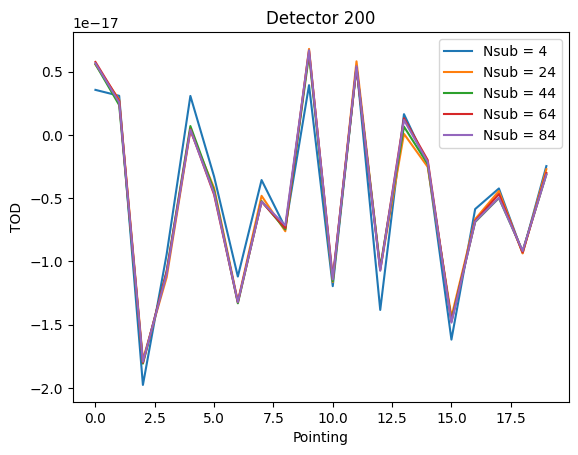
\includegraphics[width=1\linewidth]{tod_conv_one_det.png}
    \caption{TOD for a single detector of the focal plane obtained with different values of $N_{\text{sub}}$.}
    \label{fig:tod_one_det}
\end{figure}

For a more accurate characterisation, we consider a set of $N_{\text{sub}}$ values and compute the corresponding TOD for each case. From these, we define the metric :

\begin{equation}
    \delta_i = \frac{\left\| H(\mathrm{map})^{i} - H(\mathrm{map})^{\mathrm{max}} \right\|_2}{\left\| H(\mathrm{map})^{\mathrm{max}} \right\|_2},
\end{equation}

which quantifies the relative difference between the TOD obtained with a given $N_{\text{sub},i}$ and the TOD computed with the largest value $N_{\text{sub}}^{\mathrm{max}}$. The normalisation by the norm of $H(\mathrm{map})^{\mathrm{max}}$ provides a dimensionless estimate of the fractional deviation.

\subsubsection{Optimal sub-bands number for simulation and reconstruction}

Following the results obtained on the influence of $N_{\text{sub}}$ on the TOD, we consider an alternative test based on the effect of $N_{\text{sub}}$ on $\sigma_r$, the uncertainty on the tensor-to-scalar ratio $r$.
This test is, by construction, more involved, as it aims at identifying a realistic value of $N_{\text{sub}}$ for TOD generation by studying the behaviour of the uncertainty on a fitted parameter at the end of the reconstruction pipeline. We consider this metric to be particularly relevant, as it directly reflects the final objective of the simulation and reconstruction framework.
To perform this analysis, special care must be taken to distinguish the value of $N_{\text{sub}}$ used in the simulation from the one used in the reconstruction. In the following, these quantities are denoted respectively by $N_{\text{sub}}^{\mathrm{in}}$ and $N_{\text{sub}}^{\mathrm{out}}$. It is therefore necessary to investigate their respective impact on $\sigma_r$, leading to a more complete two-dimensional parameter study.

In many previous simulations (prior to this work), the same value of $N_{\text{sub}}$ was used for both simulation and reconstruction, which can introduce an artificial self-consistency between the simulated data and the reconstruction algorithm. In the present work, we avoid this condition in order to improve realism.
This study thus provides an opportunity to determine an optimal pair of parameters, both in terms of convergence of $\sigma_r$ and computational efficiency, including memory usage.

The results of this study are presented in Figure~\ref{fig:nsub_sigma_r}. The left panel shows the fit using only the two QUBIC frequency bands, while the right panel combines the QUBIC data with the $143$, $217$, and $353$ GHz frequency bands from Planck. In both cases, the figure shows the value of $\sigma_r$ for each combination of $N_{\text{sub}}^{\mathrm{in}}$ and $N_{\text{sub}}^{\mathrm{out}}$. It is reassuring to observe a similar behaviour in the two configurations.
As expected, the cases where $N_{\text{sub}}^{\mathrm{in}} = N_{\text{sub}}^{\mathrm{out}}$ yield the lowest values of $\sigma_r$, as the simulation and reconstruction are self-consistent. However, this configuration is not representative of real observations and is therefore not considered further. Excluding these cases, convergence begins to be observed for $N_{\text{sub}}^{\mathrm{in}} \gtrsim 40$ and $N_{\text{sub}}^{\mathrm{out}} \gtrsim 12$. For computational reasons, using $N_{\text{sub}}^{\mathrm{in}} = 80$ is challenging because of the memory requirements. We therefore adopt the combination $N_{\text{sub}}^{\mathrm{in}} = 40$ and $N_{\text{sub}}^{\mathrm{out}} = 16$ for all subsequent end-to-end simulations.

\begin{figure}[!htbp]
\centering
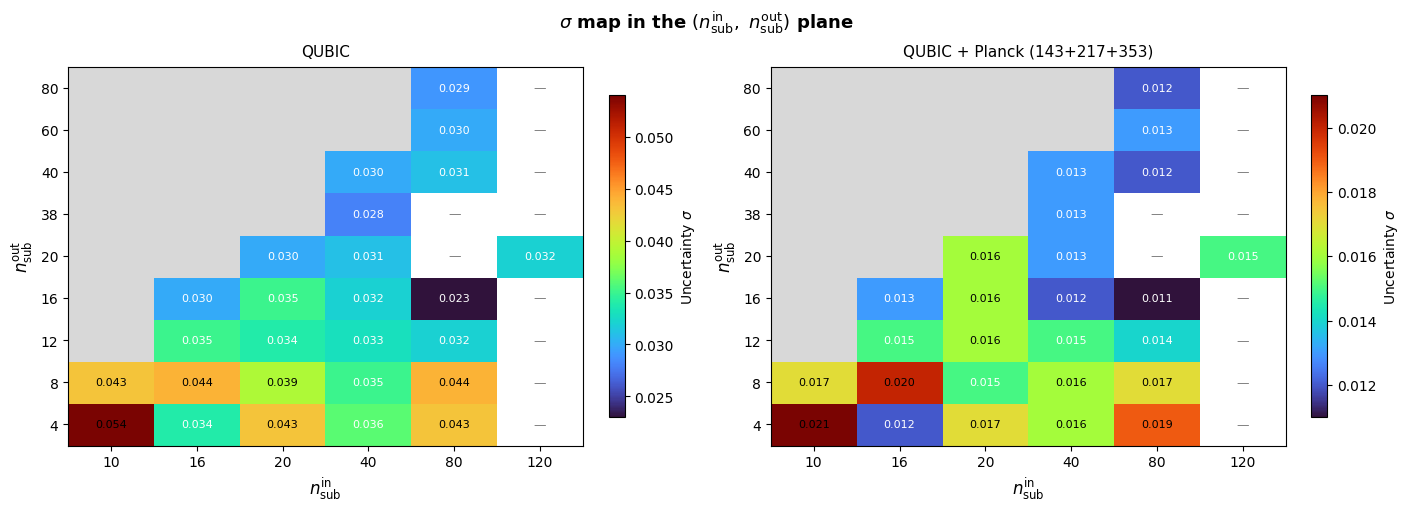
\includegraphics[width=1\linewidth]{sigma_r_nsub.png}
\caption{Uncertainty on the tensor-to-scalar ratio $r$, $\sigma_r$, for different values of $N_{\text{sub}}^{\mathrm{in}}$ used during the simulation and $N_{\text{sub}}^{\mathrm{out}}$ used during the reconstruction. Left: fit using only the two QUBIC frequency bands. Right: fit combining the QUBIC data with the $143$, $217$, and $353$ GHz Planck frequency bands.}
\label{fig:nsub_sigma_r}
\end{figure}

An additional simulation was performed for $N_{\text{sub}}^{\mathrm{in}} = 120$, which was close to the memory limit of the computing centre used for this work. This extra point confirms that the convergence observed for $N_{\text{sub}}^{\mathrm{in}} \geq 40$ is maintained at higher values.

\rmk{I still miss the point 80/38, I will run it in the following days (I had it but made a mistake...)}

\subsection{Maximum diffraction order}

The other parameter determining the realism of the simulated TOD is the maximum diffraction order $k_\text{max}$. This parameter characterises the number of peaks computed within the simulation, following $N_\text{peak} = \left(2k_\text{max} + 1\right)^2$. It is not straightforward to visualise the effect of $k_\text{max}$, which is a bit deeper than what it looks like. Given all the figures of the synthesized beam we have shown through this thesis, one can easily talk about \enquote{central peak} and \enquote{secondary peaks} to describe its structure. But, there is no such things, as the \enquote{central peak} appears only for a detector aligned with the optical axis of the instrument. In this very specific case, the order 0 peak (when $k_\text{max} = 0$, $N_\text{peak} = 1$) is located exactly at the center of the focal plane, where the primary beam is at its maximum. This situation does not happen which the real instrument, because no detector is located at the center. For an off-axis detector, the brightest peak is not located at the maximum of the primary beam, and is not necessary the order 0 peak. This situation is illustrated in Figure~\ref{fig:synth_beam_off_centre_bis}, taken from Chapter~\ref{chap:spectral_imaging}. This can be expanded further : for detectors located far from the center, an order $2$ peaks can have a higher amplitude than an order $1$ peak. For this reason, it is necessary for the realism to have a $k_\text{max}$ parameter as high as possible. 

\begin{figure}[!htbp]
    \centering
    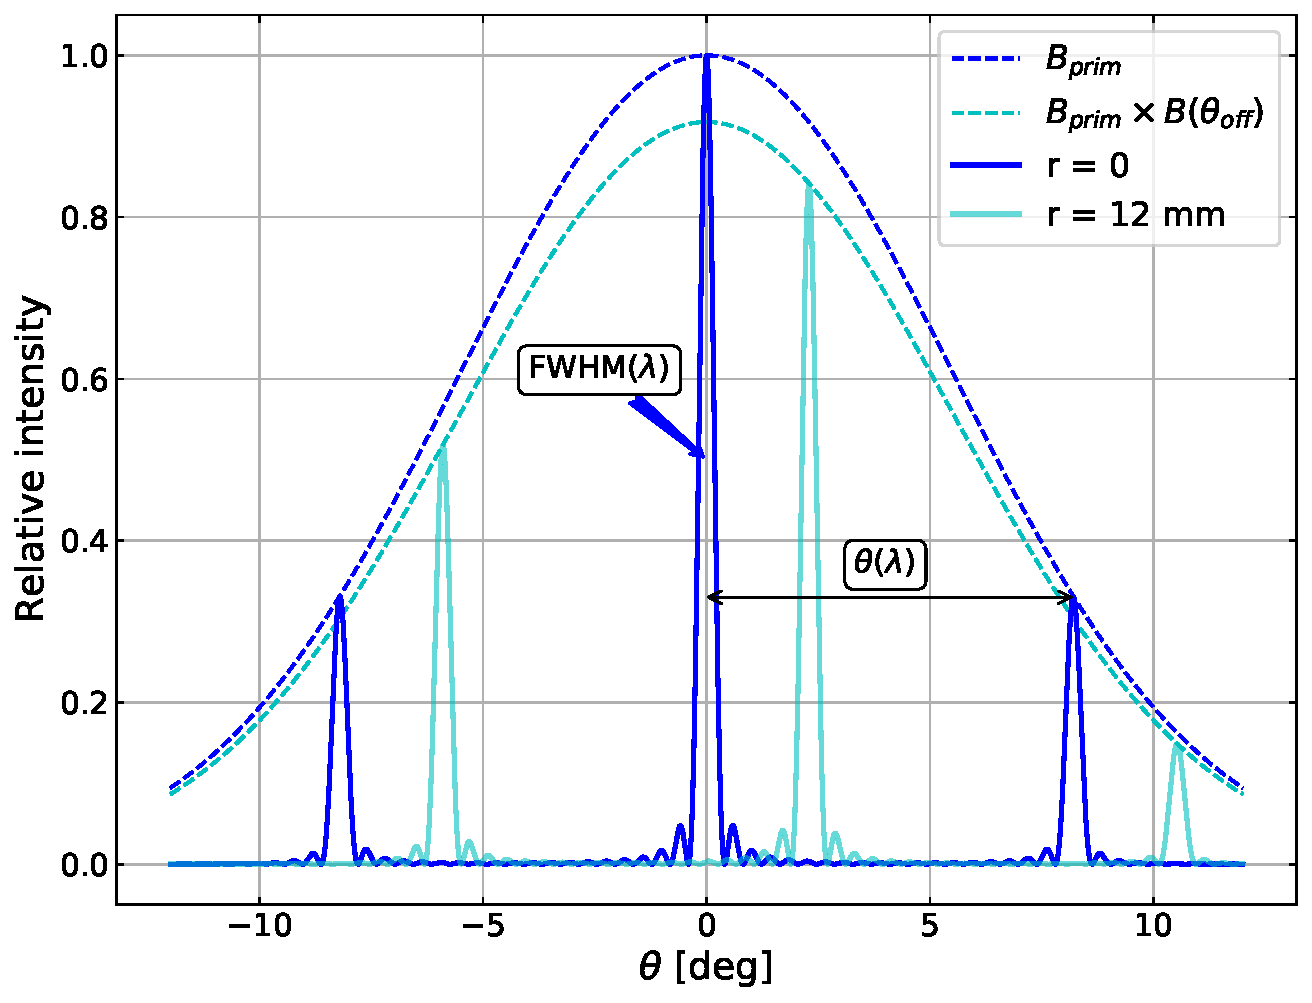
\includegraphics[width=1\linewidth]{synth_beam_off_centre.pdf}
    \caption{1D cut of the synthesized beam for two detectors: one centred on the optical axis and one off-centre by $12~\mathrm{mm}$. Taken from \cite{QUBICII}.}
    \label{fig:synth_beam_off_centre_bis}
\end{figure}

Unfortunatly, $k_\text{max}$ is a very costly parameter, the memory increasing quadratically with it. For $k_\text{max} = 1$ and $N_\text{sub} = 40$, the simulation costs already $\sim 40-50$ GB. So, it meams complicated to have a high $k_\text{max}$ while keeping a realistic $N_\text{sub}$. Therefore, we led a similar analysis to show the effect of $k_\text{max}$ on convegergence of $\sigma_r$. 
To avoid using too much memory, a parameter called \emph{synth\_beam\_fraction} was implemented. This parameter, contains between $0$ and $1$, corresponds to the fraction of the total synthesized beam amplitude we keep. To give a more practical example, the simulation is computing the amplitude associated with each peak, sort them, and keep the first ones until it reaches the \emph{synth\_beam\_fraction} value. This method allows to consider each peak, while saving memory by conserving only the ones contributing the most. This parameter is also included in our analysis.
In addition, and similarly as $N_\text{sub}$, we have to define the $k_\text{max}$ used to simulate data, noted $k_{\text{max}}^{\mathrm{in}}$, and the one used for the reconstruction $k_{\text{max}}^{\mathrm{out}}$. For realism, we impose that the \emph{synth\_beam\_fraction} associated with $k_{\text{max}}^{\mathrm{out}}$ is always equal at $1$, while the one for reconstruction can vary.

\rmk{I am still running simulation with $k_\text{max}$, it takes a lot of time, and there is a lot of things to understand that nobody did.}

\section{Simulation hyperparameters optimisation}

\subsection{Number of time samples : $N_\text{pointings}$}

The parameter $N_{\text{pointings}}$ corresponds to the number of sky observations, or equivalently the number of time samples acquired during an observation. For a real instrument acquiring data at 100 Hz, a 10-hour observation corresponds to approximately $3.6\times10^6$ pointings. As explained in Sections~\ref{subsub:fmm_memory} and~\ref{subsub:fmm_computation}, running simulations with such a large value of $N_{\text{pointings}}$ is computationally prohibitive.

To overcome this limitation, we adopt a random-pointing scanning strategy, in which the instrument points randomly within the observed patch of radius $15^\circ$. Compared to a realistic scanning strategy, this approach requires significantly fewer time samples to achieve a homogeneous angular coverage of the observed region. Consequently, a much smaller number of pointings can be used while preserving the statistical properties of the observation, resulting in simulations that remain computationally feasible. The noise level is then rescaled to match the expected observation time by defining an effective observation duration. Nevertheless, it remains necessary to determine an appropriate value for $N_{\text{pointings}}$, even within this random pointing framework.

To do so, two complementary tests were performed. The first consists of studying the evolution of the coverage as a function of $N_{\text{pointings}}$. The objective is to obtain a sufficiently uniform coverage of the observed patch. In practice, we seek the value of $N_{\text{pointings}}$ beyond which the normalised coverage no longer changes significantly, indicating convergence.

To illustrate the influence of the number of pointings on the coverage, Figure~\ref{fig:coverage_pointings} shows gnomonic projections of the QUBIC patch coverage for $N_{\text{pointings}}=100$ and $N_{\text{pointings}}=10000$. The left panel corresponds to 100 time samples and exhibits a highly inhomogeneous and asymmetric coverage pattern. In contrast, the right panel, obtained with 10000 time samples, displays a broad Gaussian-like shape with a symmetric pattern and an approximately uniform coverage at a given angular distance from the centre of the patch. This angular uniformity is particularly important, as it ensures that the coverage, and therefore the reconstruction noise, depends only on the angular distance from the patch centre.

\begin{figure}[!htbp]
    \begin{minipage}{0.5\linewidth}    
        \centerline{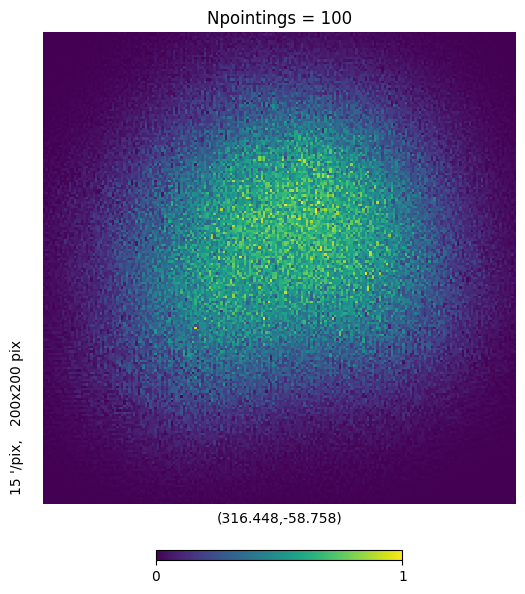
\includegraphics[width=1\linewidth]{coverage_100.png}}
    \end{minipage}
    \hfill
    \begin{minipage}{0.5\linewidth}
        \centerline{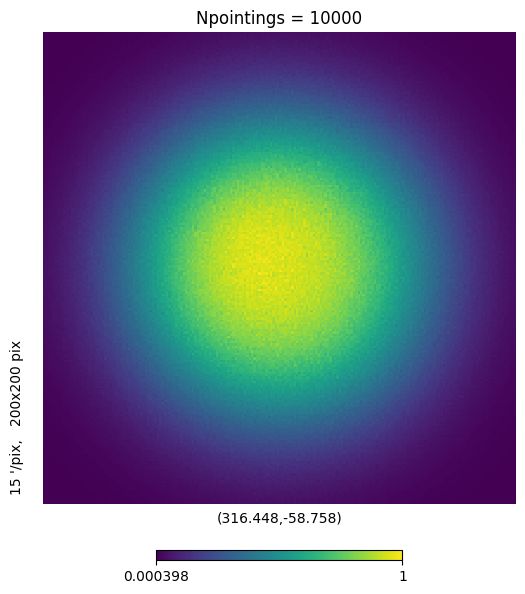
\includegraphics[width=1\linewidth]{coverage_10000.png}}
    \end{minipage}
    \caption{Gnomview of the normalised coverage of the observing patch for $N_\text{pointings} = 100$ (left) and $N_\text{pointings} = 10000$.}
    \label{fig:coverage_pointings}
\end{figure}

The coverage was then computed for various values of $N_{\text{pointings}}$, together with its angular profile and the corresponding angular RMS profile. The objective of this analysis, presented in Figure~\ref{fig:coverage_ang_profile}, is to determine the number of time samples required for convergence. The left panel shows the angular profile of the normalised coverage. One can observe that its shape converges for approximately $N_{\text{pointings}} \sim 6000$. This result is confirmed by the right panel, which displays the RMS of the normalised coverage as a function of angular distance. The RMS profile stabilises for roughly the same number of time samples, indicating that the coverage has reached convergence.

\textbf{Remark:} One may notice that the maximum value of the angular profile shown in the left panel is not equal to unity, despite the coverage being normalised. This is because each point corresponds to an average within an angular bin. For low values of $N_{\text{pointings}}$, the coverage is highly inhomogeneous, causing the bin-averaged value to differ significantly from one. The progressive convergence of the peak value towards unity therefore provides an additional indicator of convergence with increasing $N_{\text{pointings}}$.

\begin{figure}[!htbp]
    \begin{minipage}{0.5\linewidth}
        \centering
        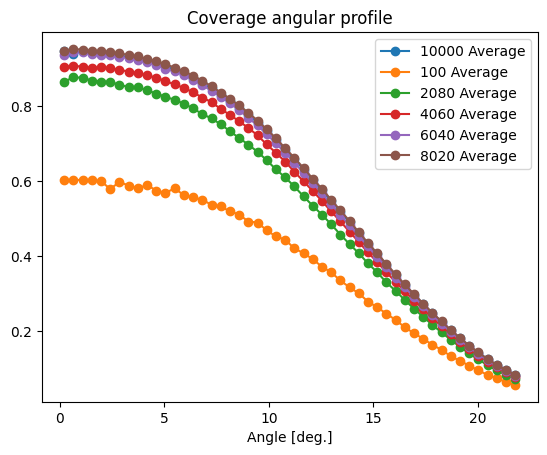
\includegraphics[width=\linewidth]{coverage_angular_profile.png}
    \end{minipage}
    \hfill
    \begin{minipage}{0.5\linewidth}
        \centering
        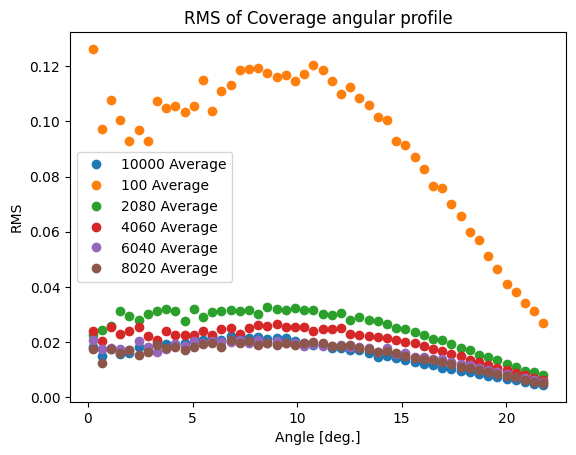
\includegraphics[width=\linewidth]{coverage_rms_angular_profile.png}
    \end{minipage}
    \caption{Angular profile (left) and RMS of the angular profile (right) of the normalised coverage for various values of $N_{\text{pointings}}$.}
    \label{fig:coverage_ang_profile}
\end{figure}

A complementary approach consists of studying the convergence of $\sigma_r$, the uncertainty on the tensor-to-scalar ratio $r$, as a function of $N_{\text{pointings}}$. This analysis is performed by running end-to-end simulations for several values of $N_{\text{pointings}}$ and fitting the resulting power spectra (see Chapter~\ref{chap:xspectrum}). The results are shown in Figure~\ref{fig:pointing_sigma_r}. The lower panel clearly shows that $\sigma_r$ converges for approximately $N_{\text{pointings}} \gtrsim 3000$.

\begin{figure}[!htbp]
    \centering
    
\includegraphics[width=1\linewidth]{sigma_r_pointings.png}
    \caption{Top: fitted value of the tensor-to-scalar ratio $r$ as a function of the number of pointings $N_{\text{pointings}}$. Error bars correspond to the MCMC uncertainty $\sigma_r$. Bottom: evolution of $\sigma_r$ as a function of $N_{\text{pointings}}$.}
    \label{fig:pointing_sigma_r}
\end{figure}

In light of these two analyses, we adopt $N_{\text{pointings}} = 5000$ for all subsequent simulations. This value provides a reasonable compromise between accuracy, memory consumption, and computational cost.

\subsection{Coverage cut}

To improve the signal-to-noise ratio, the outer pixels of the QUBIC sky patch, where the coverage is the lowest, can be excluded from the analysis. This selection is controlled by the \emph{coverage cut} parameter. Defined between 0 and 1, it corresponds to the minimum accepted coverage fraction. All pixels whose coverage fraction, defined as the coverage value at the pixel position divided by the maximum coverage over the patch, is below the chosen coverage cut are removed from the reconstruction.

Applying a coverage cut generally improves the signal-to-noise ratio by discarding poorly observed regions. However, the value should remain as small as possible in order to preserve the largest possible sky area and therefore the available statistical information. To determine an appropriate value, we follow the same procedure as in the previous section: we perform simulations for some coverage cut values and study the resulting behaviour of $\sigma_r$.

\rmk{Still miss some values for the plot.}

\subsection{Spectrum parameter : $\Delta_\ell$}

As discussed in Chapter~\ref{chap:xspectrum}, the angular power spectra are computed from $\ell_\text{min} = 40$ to $\ell_\text{max} = 2 \times N_\text{side} - 1 = 511$, with a binning given by the parameter $\Delta_\ell$.
While $\ell_\text{max}$ is limited by NaMaster, and $\ell_\text{min}$ by the size of the observing patch, it is still necessary to optimise the size of the bins.
The binning of the spectra is done for multiple purposes. The main one is to improve the signal-to-noise ratio. Indeed, when we are binning, we are averaging multiple modes into one, leading to a smaller covariance (it is divided by $\Delta_\ell$, see equation \ref{eq:xspec_noise_cov_matrix}). It also leads to a less costly fitting procedure, as we have to compute less cross-spectra value, leading to a runnable MCMC. More importantly, as we observe a small fraction of the sky, NaMaster~\cite{alonso2019} computes the spectra on a mask map. Doing so, it breaks the orthogonality of the spherical harmonics, mixing power between neighbours modes. Therefore, averaging close modes is a way to have uncorrelated power spectra with masked sky. One can note that binning is possible only because foregrounds' models evolve smoothly in $\ell$. 

As an empirical and extensive analysis was performed on the spectra parameters by Jean-Christophe Hamilton and Louise Mousset for \cite{QUBICI, QUBICII}, we decided to only test few values to compare with $\Delta_\ell = 30$ they found. We only ran simulations for $\Delta_\ell = \left[20, 30, 40, 50\right]$. The result is visible in Figure~\ref{fig:delta_ell_sigma_r}.

\begin{figure}[!htbp]
    \centering
    
\includegraphics[width=1\linewidth]{sigma_r_delta_ell.png}
    \caption{Top: fitted value of the tensor-to-scalar ratio $r$ as a function of $\Delta_\ell$. Error bars correspond to the MCMC uncertainty $\sigma_r$. Bottom: evolution of $\sigma_r$ as a function of $\Delta_\ell$.}
    \label{fig:delta_ell_sigma_r}
\end{figure}

If we look only at fit with only QUBIC (blue points), the result are very close. On the other hand, looking at the fit where high frequency bands from Planck are added (orange points), we see that the lower $\sigma_r$ is achieved with $\Delta_\ell = 30$, which confirms the previous estimation. But, we see that the fit for $\Delta_\ell = 20$ fails. This behaviour can be understood by recalling the cross-spectrum debiasing procedure described in Chapter~\ref{chap:xspectrum}. For smaller bin widths, the covariance is reduced less efficiently, increasing the sensitivity to residual noise bias. Consequently, a larger number of noise realisations is required to accurately estimate and remove this bias.

Therefore, to avoid the need to increase the already large number of realisations, and as it already shows that best performance is achieved with only QUBIC information, we decided to keep $\Delta_\ell = 30$ for our end-to-end simulations. 

\rmk{It would be good if I can add few other values (25, 35, ...), I will see if I have the time.}

\subsection{CMM convergence parameters : $N_\text{iter}$ \& $N_\text{loop}$}

In the CMM Chapter~\ref{chap:CMM}, we discussed in detail the issues related to the alternating convergence scheme used to reconstruct both the component maps and the mixing matrix (through either blind or parametric models).
This algorithm is governed by two parameters: the number of PCG iterations $N_{\mathrm{iter}}$ used to reconstruct the component maps, and the number of outer loops $N_{\mathrm{loop}}$. These two parameters must be tuned to achieve optimal convergence in the smallest possible number of steps.

The key parameter is $N_{\mathrm{iter}}$, which largely determines the convergence rate. Indeed, it controls the reconstruction accuracy of the component maps at each iteration of the outer loop. If it is too small, the maps are poorly reconstructed, and the estimation of the mixing matrix becomes biased. If it is too large, the computational cost becomes inefficient. Moreover, in the most critical case, when the mixing matrix is itself incorrectly estimated (at the beginning of the reconstruction), a large value of $N_{\mathrm{iter}}$ can lead the maps to converge towards an incorrect solution, which in turn biases the subsequent estimation of the mixing matrix. Finding the appropriate trade-off is therefore delicate and may depend on the assumed physical model of the sky.

To estimate the proper couple for these parameters, we are looking at two elements : the convergence of the spectral index, which determine the reconstruction of the mixing matrix, and the noise profile in residual component maps. 

\rmk{Still ongoing, I am doing empirical tests to understand what is the best combinaison between $N_\text{iter}$ \& $N_\text{loop}$. I made a mistake, so I have to redo simulation, but only one per case instead of 300...}

\end{document}